\documentclass[11pt, aspectratio=43]{beamer}

\usetheme{Madrid}
\usecolortheme{default}

\usepackage{graphicx}
\usepackage{amsmath}
\usepackage{amsfonts}
\usepackage{amssymb}
\usepackage{booktabs}
\usepackage{textcomp}
\usepackage{array}
\usepackage{colortbl}
\usepackage{xcolor}
\usepackage{parskip}

% Custom colors for tables
\definecolor{posgreen}{RGB}{0,128,0}
\definecolor{negred}{RGB}{180,0,0}
\definecolor{headerblue}{RGB}{51,51,153}
\definecolor{lightgray}{RGB}{240,240,240}

\title[MS5610 Presentation]{Fund Performance and Analysis}
\author{Group 8}
\date{\today}

\begin{document}

\begin{frame}
    \titlepage
\end{frame}

\begin{frame}{Outline}
    \tableofcontents
\end{frame}

%% ===================================================================
\section{UTI Large \& Mid Cap Fund} %Neeraja
%% ===================================================================

\begin{frame}{}
\centering
\vspace{2em}
{\huge UTI Large \& Mid Cap Fund}

\vspace{1.5em}
{\large Analysis by Neeraja}
 
\end{frame}

\begin{frame}{About Fund}
\begin{itemize}
    \item \textbf{Fund Name:} UTI Large \& Mid Cap Fund (Direct Plan -- Growth)
    \item \textbf{Benchmark:} Nifty LargeMidcap 250 TRI
    \item \textbf{AUM:} Rs.\ 6,406.53 crore (as on 30 June 2026)
    \item \textbf{NAV:} Rs.\ 200.83 (Direct Plan -- Growth, as on 31 July 2026)
    %\item \textbf{Fund Manager:} V.\ Srivatsa
    \item \textbf{Major Constituent:} HDFC Bank Ltd ($\sim$5.49\%)
    \item \textbf{Holdings:} 70 stocks; 95.44\% equity, $\sim$4.56\% cash \& other
\end{itemize}
\end{frame}


\begin{frame}{Fund Performance}
\centering
\small
\begin{tabular}{l r}
\toprule
\textbf{Measure} & \textbf{Value} \\
\midrule
Mean Daily Excess Return ($\bar{R}_p - R_f$) & 0.0418\% \\
Std Dev (Total Risk, $\sigma_p$) & 0.7006\% \\
CAPM Beta ($\beta$) & 0.9663 \\
CAPM $R^2$ & 0.9201 \\
\midrule
Sharpe Ratio (annualized) & 1.0592 \\
Treynor Ratio (annualized) & 12.19\% \\
Jensen's Alpha (annualized) & 10.67\% \\
Information Ratio (annualized) & $-$2.1182 \\
Tracking Error (annualized) & 3.1664\% \\
\bottomrule
\end{tabular}

\vspace{0.5em}
\footnotesize
July 2026 daily data (n=22). $R_f$ = daily equivalent of 6\% annual risk-free rate.
\end{frame}


\begin{frame}{Fama-French Three-Factor Regression}
\centering
\small
$R_i - R_f = \alpha + \beta(R_m - R_f) + \delta \cdot \text{SMB} + \lambda \cdot \text{HML} + \varepsilon$

\vspace{0.5em}
\begin{tabular}{l r r r}
\toprule
\textbf{Variable} & \textbf{Coefficient} & \textbf{t-stat} & \textbf{p value} \\
\midrule
Mkt Excess ($\beta$) & 0.9368 & \textbf{15.444}$^{**}$ & 0.0000 \\
SMB ($\delta$) & 0.0004 & 0.397 & 0.6899\\
HML ($\lambda$) & $-$0.0027 & \textbf{$-$2.498}$^{**}$ & 0.0218\\
Intercept ($\alpha$) & $-$0.0001 & $-$0.256 & 0.8004 \\
\midrule
$R^2$ & \multicolumn{3}{c}{0.9406} \\
F-statistic & \multicolumn{3}{c}{100.29} \\
Residual d.f. & \multicolumn{3}{c}{19} \\
\bottomrule
\end{tabular}

\vspace{0.5em}
\footnotesize
$^{**}|t|>2.1$ at 5\% level (d.f.=19). Market and HML are significant --- a mild
value tilt shows up once size/value are separated out; size (SMB) loading is
negligible.
\end{frame}


\begin{frame}{Carhart's Four-Factor Regression}
\centering
\small
$R_i - R_f = \alpha + \beta(R_m - R_f) + \delta \cdot \text{SMB} + \lambda \cdot \text{HML} + \rho \cdot \text{MOM} + \varepsilon$

\vspace{0.5em}
\begin{tabular}{l r r r}
\toprule
\textbf{Variable} & \textbf{Coefficient} & \textbf{t-stat} & \textbf{p value}\\
\midrule
Mkt Excess ($\beta$) & 0.9877 & \textbf{13.480}$^{**}$ & 0.0000\\
SMB ($\delta$) & $-$0.0000 & $-$0.040 & 0.9684\\
HML ($\lambda$) & $-$0.0031 & \textbf{$-$2.780}$^{**}$ & 0.0119\\
MOM ($\rho$) & $-$0.0011 & $-$1.209 & 0.2416 \\
Intercept ($\alpha$) & $-$0.0001 & $-$0.347 & 0.7322 \\
\midrule
$R^2$ & \multicolumn{3}{c}{0.9451} \\
F-statistic & \multicolumn{3}{c}{77.41} \\
Residual d.f. & \multicolumn{3}{c}{18} \\
\bottomrule
\end{tabular}

\vspace{0.5em}
\footnotesize
$^{**}|t|>2.1$ at 5\% (d.f.=18). Market and HML remain significant; momentum
is directionally negative but not significant. Alpha is statistically zero
once all four factors are controlled for.
\end{frame}


\begin{frame}{Portfolio Style Evaluation}
\centering
\small
$R_{\text{fund}} = \alpha + \beta \cdot R_{\text{market}} + \varepsilon$

\vspace{0.5em}

\begin{tabular}{l r r r}
\toprule
\textbf{Parameter} & \textbf{Value} & \textbf{Std Error} & \textbf{t-stat} \\
\midrule
Alpha (Security Selection) & $-$0.0002 & 0.0004 & $-$0.447 \\
Beta (Market Timing) & 0.9663 & 0.0622 & \textbf{15.546}$^{**}$ \\
$R^2$ & \multicolumn{3}{c}{0.9201} \\
\bottomrule
\end{tabular}

\vspace{0.8em}
\begin{itemize}
    \small
    \item \textbf{Security Selection} ($\alpha = -0.0002$): Negative but insignificant --- no evidence of superior stock picking at the single-factor level.
    \item \textbf{Market Timing} ($\beta = 0.966$): Essentially market-matching, marginally defensive. Structural, not tactical.
    \item \textbf{$R^2 = 92.0\%$}: Very high for a 70-stock large \& midcap fund. The $\sim$8\% residual reflects off-benchmark sector tilts (Banks overweight, Auto Components/Electrical Equipment underweight).
\end{itemize}
\end{frame}


\begin{frame}{Sector Attribute Analysis (Brinson--Fachler)}
\centering
\footnotesize
\begin{tabular}{l r r r r}
\toprule
\textbf{Sector} & \textbf{Allocation} & \textbf{Selection} & \textbf{Interaction} & \textbf{Total} \\
\midrule
\rowcolor{lightgray}
IT -- Software & \textcolor{posgreen}{+0.33\%} & +0.04\% & +0.02\% & \textcolor{posgreen}{\textbf{+0.39\%}} \\
Non -- Ferrous Metals & $-$0.00\% & \textcolor{posgreen}{+0.15\%} & +0.02\% & \textcolor{posgreen}{\textbf{+0.17\%}} \\
\rowcolor{lightgray}
Electrical Equipment & \textcolor{posgreen}{+0.33\%} & \textcolor{negred}{$-$0.57\%} & +0.41\% & \textcolor{posgreen}{\textbf{+0.17\%}} \\
Industrial Products & +0.11\% & +0.06\% & $-$0.05\% & \textcolor{posgreen}{\textbf{+0.11\%}} \\
\rowcolor{lightgray}
Auto Components & $-$0.02\% & \textcolor{negred}{$-$0.36\%} & +0.25\% & \textcolor{negred}{\textbf{$-$0.13\%}} \\
Banks & \textcolor{negred}{$-$0.13\%} & $-$0.05\% & $-$0.02\% & \textcolor{negred}{\textbf{$-$0.20\%}} \\
\rowcolor{lightgray}
Consumer Durables & \textcolor{negred}{$-$0.15\%} & \textcolor{negred}{$-$0.41\%} & +0.28\% & \textcolor{negred}{\textbf{$-$0.28\%}} \\
Pharma \& Biotech & +0.07\% & \textcolor{negred}{$-$0.32\%} & $-$0.14\% & \textcolor{negred}{\textbf{$-$0.39\%}} \\
\midrule
\textbf{Total (all sectors)} & \textbf{+0.42\%} & \textbf{$-$1.62\%} & \textbf{+0.94\%} & \textbf{$-$0.25\%} \\
\bottomrule
\end{tabular}

\vspace{0.5em}
\footnotesize
Fund weighted return: 1.73\% \quad|\quad Benchmark weighted return: 2.00\%
\end{frame}


\begin{frame}{Sector Attribute Analysis --- Key Findings}
\begin{itemize}
    \small
    \item \textcolor{posgreen}{\textbf{IT -- Software (+0.39\%)}}: Largest positive contributor. Fund overweighted the sector (7.72\% vs 5.16\%), which itself rallied 14.86\%, and the fund's own IT names beat even that at 15.66\%. Strong allocation \textit{and} selection.
    \item \textcolor{posgreen}{\textbf{Electrical Equipment (+0.17\%)}}: Fund stayed sharply underweight (1.33\% vs 4.73\%) in a sector that fell $-$7.63\% -- smart avoidance. But the few names it did hold collapsed $-$19.76\%, so the win came entirely from timing, not picking.
    \item \textcolor{posgreen}{\textbf{Non-Ferrous Metals (+0.17\%)}}: A small, well-picked position -- fund holdings returned 12.69\% against a near-flat 1.06\% sector average. Pure security-selection win.
    \item \textcolor{negred}{\textbf{Pharma \& Biotech ($-$0.39\%)}}: Largest drag. Fund correctly overweighted (8.72\% vs 6.02\%) a sector that beat the portfolio average, but its own pharma names lost $-$0.6\% against a 4.75\% sector average -- a costly stock-picking miss (Divi's Labs, +21.0\%, was available and underused).
    \item \textcolor{negred}{\textbf{Banks ($-$0.20\%)}}: A 4.48-point overweight (15.94\% vs 11.46\%) into a sector that underperformed ($-$0.8\% vs +2.0\% portfolio average) -- the single largest wrong-way sector bet.
\end{itemize}
\end{frame}


\begin{frame}{Hypothetical Allocation }
\centering
\footnotesize
\resizebox{\textwidth}{!}{%
\begin{tabular}{l c c l}
\toprule
\textbf{Sector} & \textbf{Actual Wt} & \textbf{Proposed Wt} & \textbf{Rationale} \\
\midrule
Banks & 15.94\% & $\sim$11.5\% & Cut the largest wrong-way overweight \\
IT -- Software & 7.72\% & $\sim$10.3\% & Ride the sector's 14.86\% rally further \\
Consumer Durables & 1.10\% & $\sim$3.3\% & Match benchmark; missed an 8.67\% rally \\
Auto Components & 0.86\% & $\sim$2.9\% & Match benchmark; missed a rallying sector \\
Pharma \& Biotech & 8.72\% & $\sim$6.0\% & Trim; overweight amplified poor stock picks \\
\bottomrule
\end{tabular}%
}

\vspace{0.8em}
\begin{tabular}{l r}
\toprule
\textbf{Metric} & \textbf{Value} \\
\midrule
Actual Fund Weighted Return & 1.73\% \\
Proposed Fund Weighted Return & 1.95\% \\
\textbf{Improvement from Reallocation} & \textbf{+0.22\%} \\
\bottomrule
\end{tabular}

\vspace{0.5em}
\footnotesize
\textit{Assumption: Individual security returns unchanged; only sector allocation weights adjusted.}
\end{frame}


%% ===================================================================
\section{Invesco India Largecap Fund} %Lokesh
%% ===================================================================

\begin{frame}{}
\centering
\vspace{2em}
{\huge Invesco India Large Cap Fund}

\vspace{1.5em}
{\large Analysis by Lokesh}
 
\end{frame}

\begin{frame}{About Fund}
\begin{itemize}
    \item \textbf{Fund Name:} Invesco India Largecap Fund (Regular Plan -- Growth)
    \item \textbf{Benchmark:} Nifty 100 TRI
    \item \textbf{AUM:} Rs.\ 1,931.4 crore (as on 31 July 2026)
    \item \textbf{NAV:} Rs.\ 88.13 (Direct Plan -- Growth)
    % \item \textbf{Fund Manager:} Hiten Jain (17 years experience)
    \item \textbf{Major Constituent:} ICICI Bank Ltd ($\sim$8.25\%)
    \item \textbf{Holdings:} 55 stocks; 99.46\% equity, 0.54\% cash
\end{itemize}
\end{frame}


\begin{frame}{Fund Performance}
\centering
\small
\begin{tabular}{l r}
\toprule
\textbf{Measure} & \textbf{Value} \\
\midrule
Mean Daily Excess Return ($\bar{R}_p - R_f$) & 0.0738\% \\
Std Dev (Total Risk, $\sigma_p$) & 0.7697\% \\
CAPM Beta ($\beta$) & 1.0372 \\
CAPM $R^2$ & 0.8839 \\
\midrule
\textbf{Sharpe Ratio} (annualized) & \textbf{1.5228} \\
\textbf{Treynor Ratio} (annualized) & \textbf{17.94\%} \\
\textbf{Jensen's Alpha} (annualized) & \textbf{$-$10.14\%} \\
\textbf{Information Ratio} (annualized) & \textbf{$-$2.3048} \\
\textbf{Tracking Error} (annualized) & \textbf{4.18\%} \\
\bottomrule
\end{tabular}

\vspace{0.8em}
\footnotesize
\textit{July 2026 daily data (n=22). $R_f$ = daily equivalent of 5.41\% MIBOR.}
\end{frame}

\begin{frame}{Fama-French Three-Factor Regression}
\centering
\small
$R_i - R_f = \alpha + \beta(R_m - R_f) + \delta \cdot SMB + \lambda \cdot HML + \varepsilon$

\vspace{0.5em}

\begin{tabular}{l r r r}
\toprule
\textbf{Variable} & \textbf{Coefficient} & \textbf{t-stat} & \textbf{p-value} \\
\midrule
Mkt Excess ($\beta$) & 1.0444 & \textbf{9.849}$^{**}$ & $<$0.0001 \\
SMB ($\delta$) & 0.0656 & 0.526 & 0.6053 \\
HML ($\lambda$) & $-$0.0581 & $-$0.317 & 0.7549 \\
Intercept ($\alpha$) & $-$0.0004 & $-$0.579 & 0.5698 \\
\midrule
$R^2$ & \multicolumn{3}{c}{0.8866} \\
F-statistic & \multicolumn{3}{c}{46.91} \\
Residual d.f. & \multicolumn{3}{c}{18} \\
\bottomrule
\end{tabular}

\vspace{0.5em}
\footnotesize
$^{**}p < 0.05$. Only the market factor is significant; size and value loadings are negligible for this large-cap fund.
\end{frame}


\begin{frame}{Carhart's Four-Factor Regression}
\centering
\small
$R_i - R_f = \alpha + \beta(R_m - R_f) + \delta \cdot SMB + \lambda \cdot HML + \rho \cdot MOM + \varepsilon$

\vspace{0.5em}

\begin{tabular}{l r r r}
\toprule
\textbf{Variable} & \textbf{Coefficient} & \textbf{t-stat} & \textbf{p-value} \\
\midrule
Mkt Excess ($\beta$) & 1.0085 & \textbf{11.563}$^{**}$ & $<$0.0001 \\
SMB ($\delta$) & $-$0.0968 & $-$0.850 & 0.4071 \\
HML ($\lambda$) & 0.0684 & 0.443 & 0.6634 \\
MOM ($\rho$) & 0.2807 & \textbf{3.173}$^{**}$ & 0.0056 \\
Intercept ($\alpha$) & $-$0.0000 & $-$0.024 & 0.9811 \\
\midrule
$R^2$ & \multicolumn{3}{c}{0.9288} \\
F-statistic & \multicolumn{3}{c}{55.42} \\
Residual d.f. & \multicolumn{3}{c}{17} \\
\bottomrule
\end{tabular}

\vspace{0.5em}
\footnotesize
$^{**}p < 0.05$. Market and momentum are significant. The fund has meaningful momentum exposure ($\rho = 0.28$). Alpha is statistically zero.
\end{frame}


\begin{frame}{Portfolio Style Evaluation}
\centering
\small
$R_{\text{fund}} = \alpha + \beta \cdot R_{\text{market}} + \varepsilon$

\vspace{0.5em}

\begin{tabular}{l r r r}
\toprule
\textbf{Parameter} & \textbf{Value} & \textbf{t-stat} & \textbf{p-value} \\
\midrule
Alpha (Security Selection) & $-$0.0004 & $-$0.740 & 0.4679 \\
Beta (Market Timing) & 1.0372 & \textbf{12.341}$^{**}$ & $<$0.0001 \\
$R^2$ & \multicolumn{3}{c}{0.8839} \\
\bottomrule
\end{tabular}

\vspace{0.8em}
\begin{itemize}
    \small
    \item \textbf{Security Selection} ($\alpha = -0.0004$, $p=0.468$): Negative but insignificant --- no evidence of superior stock picking at the single-factor level.
    \item \textbf{Market Timing} ($\beta = 1.037$, $p<0.0001$): Marginally aggressive stance; amplifies market moves slightly. Structural, not tactical.
    \item \textbf{$R^2 = 88.4\%$}: High for a large-cap fund. The $\sim$12\% residual reflects off-benchmark bets (Capital Markets overweight, mid/small-cap tilt).
\end{itemize}
\end{frame}

\begin{frame}{Sector Attribute Analysis (Brinson--Fachler)}
\centering
\footnotesize
\begin{tabular}{l r r r r}
\toprule
\textbf{Sector} & \textbf{Allocation} & \textbf{Selection} & \textbf{Interaction} & \textbf{Total} \\
\midrule
\rowcolor{lightgray}
Retailing & $-$0.15\% & \textcolor{posgreen}{+0.41\%} & +0.24\% & \textcolor{posgreen}{\textbf{+0.50\%}} \\
Capital Markets & \textcolor{negred}{$-$0.35\%} & 0.00\% & 0.00\% & \textcolor{negred}{\textbf{$-$0.35\%}} \\
\rowcolor{lightgray}
Pharma \& Biotech & +0.01\% & \textcolor{posgreen}{+0.31\%} & +0.02\% & \textcolor{posgreen}{\textbf{+0.34\%}} \\
Power & \textcolor{posgreen}{+0.30\%} & 0.00\% & 0.00\% & \textcolor{posgreen}{\textbf{+0.30\%}} \\
\rowcolor{lightgray}
Oil \& Gas & +0.13\% & 0.00\% & +0.16\% & \textcolor{posgreen}{\textbf{+0.29\%}} \\
IT -- Software & \textcolor{posgreen}{+0.38\%} & $-$0.11\% & $-$0.03\% & \textcolor{posgreen}{\textbf{+0.25\%}} \\
\rowcolor{lightgray}
Healthcare Svc. & $-$0.06\% & \textcolor{negred}{$-$0.10\%} & $-$0.07\% & \textcolor{negred}{\textbf{$-$0.23\%}} \\
Automobiles & $-$0.02\% & \textcolor{posgreen}{+0.22\%} & $-$0.01\% & \textcolor{posgreen}{\textbf{+0.19\%}} \\
\midrule
\textbf{Total (all sectors)} & \textbf{+0.14\%} & \textbf{+0.98\%} & \textbf{+0.24\%} & \textbf{+1.37\%} \\
\bottomrule
\end{tabular}

\vspace{0.5em}
\footnotesize
Fund weighted return: 4.23\% \quad|\quad Benchmark weighted return: 3.12\%
\end{frame}


\begin{frame}{Sector Attribute Analysis --- Key Findings}
\begin{itemize}
    \small
    \item \textcolor{posgreen}{\textbf{Retailing (+0.50\%)}}: Largest positive contributor. Fund overweighted Eternal Ltd (Zomato, +14.30\%) vs benchmark drag from Trent ($-$8.43\%). Strong security selection \textit{and} allocation.
    \item \textcolor{posgreen}{\textbf{Pharma (+0.34\%)}}: Torrent Pharma (10.88\%) and Divi's (22.96\%) sharply outperformed the benchmark sector average (6.66\%). Pure security selection win.
    \item \textcolor{posgreen}{\textbf{Power (+0.30\%)}}: Fund dramatically underweighted this negative-return sector (0.47\% vs 5.98\%), avoiding the $-$2.27\% benchmark drag.
    \item \textcolor{negred}{\textbf{Capital Markets ($-$0.35\%)}}: Largest drag. Fund held 8.13\% vs 0.44\% benchmark weight in a sector that returned $-$1.41\%.
    \item \textcolor{negred}{\textbf{Healthcare Services ($-$0.23\%)}}: Fund overweighted (3.27\% vs 0.87\%) but the sector underperformed. Poor selection (Max Healthcare).
\end{itemize}
\end{frame}


\begin{frame}{Hypothetical Allocation --- ``If I Were the Fund Manager''}
\centering
\footnotesize
\begin{tabular}{l c c l}
\toprule
\textbf{Sector} & \textbf{Actual Wt} & \textbf{Proposed Wt} & \textbf{Rationale} \\
\midrule
Capital Markets & 8.13\% & $\sim$2.6\% & Cut largest negative active bet \\
IT -- Software & 9.37\% & $\sim$18.2\% & Ride 17.56\% sector momentum \\
FMCG & 0.00\% & $\sim$5.2\% & Add absent defensive exposure \\
Pharma & 4.43\% & $\sim$9.1\% & Double down on proven selection \\
Healthcare Svc. & 3.27\% & $\sim$1.3\% & Reduce; Max Healthcare drag \\
\bottomrule
\end{tabular}

\vspace{0.8em}
\begin{tabular}{l r}
\toprule
\textbf{Metric} & \textbf{Value} \\
\midrule
Actual Fund Weighted Return & 4.23\% \\
Proposed Fund Weighted Return & 6.36\% \\
\textbf{Improvement from Reallocation} & \textbf{+2.13\%} \\
\bottomrule
\end{tabular}

\vspace{0.5em}
\footnotesize
\textit{Assumption: Individual security returns unchanged; only sector allocation weights adjusted.}
\end{frame}


%% ===================================================================
\section{ICICI Prudential Small Cap Fund} %Ajith
%% ===================================================================

\begin{frame}{}
\centering
\vspace{2em}
{\huge ICICI Prudential Small Cap Fund}

\vspace{1.5em}
{\large Analysis by Ajith}

\end{frame}

\begin{frame}{About Fund}
\begin{itemize}
    \item \textbf{Fund Name:} ICICI Prudential Smallcap Fund
    \item \textbf{Benchmark:} Nifty Smallcap 250
    \item \textbf{AUM:} Rs.\ 1,273.22 crore
    \item \textbf{NAV:} Rs.\ 103.95
    \item \textbf{Average Daily Return:} 0.0327\%
    % \item \textbf{Major Constituent:} \textit{Not reported in the supplied source}
\end{itemize}
\end{frame}

\begin{frame}{Fund Performance}
\centering
\small
\begin{tabular}{l r p{4.8cm}}
\toprule
\textbf{Measure} & \textbf{Value} & \textbf{Interpretation} \\
\midrule
Sharpe Ratio & 0.1871 & Positive risk-adjusted return \\
Treynor Ratio & 3.07\% & Small positive return for systematic risk \\
Jensen's Alpha & $-$1.01\% & Negative alpha indicates underperformance versus CAPM-expected return \\
Information Ratio & $-$0.3766 & Negative active performance \\
\bottomrule
\end{tabular}

% \vspace{0.5em}
% \footnotesize
% \textit{Values reproduced from the supplied ICICI Prudential source slides; the source does not state a common annualization basis.}
\end{frame}

\begin{frame}{Fama-French Three-Factor Regression}
\centering
\small
$R_i - R_f = \alpha + \beta(R_m - R_f) + \delta \cdot SMB + \lambda \cdot HML + \varepsilon$

\vspace{0.5em}

\begin{tabular}{l r r c}
\toprule
\textbf{Factor} & \textbf{Coefficient} & \textbf{p-value} & \textbf{Significant?} \\
\midrule
Mkt Excess ($\beta$) & 0.736 & $<0.05$ & Yes \\
SMB ($\delta$) & 0.0107 & 0.313 & No \\
HML ($\lambda$) & $-$3.952 & 0.002 & Yes \\
Alpha($\alpha$) & 1.566 & 0.002 & Yes\\
\midrule
$R^2$ & \multicolumn{3}{c}{93.71\%} \\

\bottomrule
\end{tabular}

\vspace{0.5em}
\footnotesize
Market and value factors are significant; the size (SMB) loading is not distinguishable from zero. 
\end{frame}

\begin{frame}{Carhart's Four-Factor Regression}
\centering
\small
$R_i - R_f = \alpha + \beta(R_m - R_f) + \delta \cdot SMB + \lambda \cdot HML + \rho \cdot MOM + \varepsilon$

\vspace{0.5em}

\begin{tabular}{l r r c}
\toprule
\textbf{Factor} & \textbf{Coefficient} & \textbf{p-value} & \textbf{Significant?} \\
\midrule
Mkt Excess ($\beta$) & 0.738 & $<0.05$ & Yes \\
SMB ($\delta$) & 0.338 & 0.222 & No \\
HML ($\lambda$) & $-$3.812 & 0.003 & Yes \\
MOM ($\rho$) & 0.224 & 0.360 & No \\
Alpha($\alpha$) & 1.521 & 0.003 & Yes\\
\midrule
$R^2$ & \multicolumn{3}{c}{94.02\%} \\
\bottomrule
\end{tabular}

\vspace{0.5em}
\footnotesize
Adding momentum raises $R^2$ only marginally (93.71\% $\to$ 94.02\%), and MOM itself is insignificant. Market and value remain the two significant factors. 
\end{frame}

\begin{frame}{Hypothetical Manager: Sector Allocation}
\textbf{Objective:} Identify sectors where the manager should have increased or reduced exposure.

\vspace{0.4em}
\centering
\footnotesize
\begin{tabular}{l l}
\toprule
\textbf{Decision Rule} & \textbf{Condition} \\
\midrule
\textcolor{posgreen}{\textbf{BUY}} & Fund underweight \textbf{+} sector outperformed benchmark \\
\textcolor{negred}{\textbf{SELL}} & Fund overweight \textbf{+} sector underperformed benchmark \\
\textbf{NO REVISION} & Neither condition satisfied \\
\bottomrule
\end{tabular}

\vspace{0.8em}
\begin{tabular}{l r r r c}
\toprule
\textbf{Sector} & \textbf{Fund Wt} & \textbf{Sector Ret} & \textbf{Bmk TRI} & \textbf{Decision} \\
\midrule
Drugs \& Pharmaceuticals & 2.70\% & 1.67\% & 1.28\% & \textcolor{posgreen}{\textbf{BUY}} \\
Health Services & 2.39\% & 4.81\% & 1.28\% & \textcolor{posgreen}{\textbf{BUY}} \\
Boilers \& Turbines & 1.51\% & $-$12.99\% & 1.28\% & \textcolor{negred}{\textbf{SELL}} \\
Hotels \& Restaurants & 4.00\% & 0.71\% & 1.28\% & \textcolor{negred}{\textbf{SELL}} \\
\bottomrule
\end{tabular}

\vspace{0.6em}
\footnotesize
Flags sectors where the fund was underweight in an outperforming sector, or overweight in an underperforming one, relative to the benchmark.
\end{frame}

\begin{frame}{Hypothetical Manager: Security Selection}
\textbf{Objective:} Determine whether the manager selected the right securities within sectors.

\vspace{0.4em}
\centering
\footnotesize
\begin{tabular}{l l}
\toprule
\textbf{Decision Rule} & \textbf{Condition} \\
\midrule
\textcolor{posgreen}{\textbf{BUY}} & Security underweight \textbf{+} outperformed industry benchmark \\
\textcolor{negred}{\textbf{SELL}} & Security overweight \textbf{+} underperformed industry benchmark \\
\textbf{NO REVISION} & Neither condition satisfied \\
\bottomrule
\end{tabular}

\vspace{0.8em}
\begin{tabular}{l r r r c}
\toprule
\textbf{Security} & \textbf{Fund Wt} & \textbf{Security Ret} & \textbf{Industry Bmk} & \textbf{Decision} \\
\midrule
Minda Corporation & 0.33\% & 0.60\% & 3.39\% & \textcolor{negred}{\textbf{SELL}} \\
CIE Automotive & 0.34\% & $-$10.75\% & 3.39\% & \textcolor{negred}{\textbf{SELL}} \\
Aavas Financiers & 0.24\% & $-$10.59\% & $-$3.64\% & \textcolor{negred}{\textbf{SELL}} \\
Kaynes Technology & 0.41\% & 21.87\% & 3.07\% & \textbf{NO REVISION} \\
\bottomrule
\end{tabular}
\end{frame}

\begin{frame}{Proposed Portfolio Allocation}

\textbf{Manager Action}
\begin{itemize}
    \item Increase: Pharma, Healthcare Services, ITES, Housing Construction
    \item Reduce: Boilers \& Turbines, General Machinery, Hotels \& Restaurants, Securities Broking
    \item Maintain: Selected sectors with “No Revision”
    
\end{itemize}

\textbf{Impact}
\begin{itemize}
\item Current matched-sector contribution: 0.18\%
\item Proposed contribution: 0.77\%
\item Improvement: +0.59 percentage points
\end{itemize}
    
\end{frame}

\begin{frame}{Sector Attribute Analysis --- Overall Results}
\centering
\small
\begin{tabular}{l r}
\toprule
\textbf{Attribution Component} & \textbf{Value} \\
\midrule
Allocation Attribution & \textbf{+9.9033 pp} \\
Security Selection Attribution & \textbf{+1.9032 pp} \\
\bottomrule
\end{tabular}

\vspace{1em}
\begin{itemize}
    \small
    \item The allocation effect (\textbf{+9.90 pp}) is substantially larger than the security-selection effect (\textbf{+1.90 pp}).
    \item Sector-level positioning --- rather than individual stock picking --- was the dominant driver of the fund's active performance in this analysis.
\end{itemize}
\end{frame}

\section{HDFC Small Cap Fund} %Balaji
%% ===================================================================

\begin{frame}{}
\centering
\vspace{2em}
{\huge HDFC Small Cap Fund}

\vspace{1.5em}
{\large Analysis by Balaji}

\end{frame}

\begin{frame}{About Fund}
\begin{itemize}
    \item \textbf{Fund Name:} HDFC Small Cap Fund --- Direct Plan -- Growth Option
    \item \textbf{Benchmark:} BSE 250 SmallCap Index (TRI)
    \item \textbf{AUM:} Rs.\ 41,679.00 crore (31 July 2026)
    \item \textbf{NAV:} Rs.\ 160.752 (Direct Plan -- Growth; 31 July 2026)
    \item \textbf{Fund Manager:} Chirag Setalvad
    \item \textbf{Major Constituent:} Firstsource Solutions Ltd. (4.24\% of NAV)
\end{itemize}
\end{frame}

\begin{frame}{Fund Performance}
\centering
\small
\begin{tabular}{l r l}
\toprule
\textbf{Measure} & \textbf{Value} & \textbf{Basis} \\
\midrule
Fund Return (July 2026) & 2.4113\% & NAV-to-NAV \\
Benchmark Return (July 2026) & 0.3961\% & BSE 250 SmallCap TRI \\
Active Return & 2.0152\% & Fund minus benchmark \\
Mean Daily Excess Return & 0.0969\% & Over 6\% annual RF \\
Daily Return Std. Dev. & 1.6813\% & Daily fund returns \\
CAPM Beta & 0.8727 & Daily July data \\
CAPM $R^2$ & 0.9371 & Daily July data \\
\midrule
\textbf{Sharpe Ratio} & \textbf{0.0982} & Daily \\
\textbf{Sharpe Ratio} & \textbf{1.5593} & Annualized presentation \\
\textbf{Treynor Ratio} & \textbf{0.0010108} & Daily \\
\textbf{Treynor Ratio} & \textbf{25.4712\%} & Annualized presentation \\
\textbf{Jensen's Alpha} & \textbf{0.0969\%} & Daily \\
\textbf{Jensen's Alpha} & \textbf{24.4197\%} & Annualized presentation \\
\textbf{Information Ratio} & \textbf{0.3799} & Active return / tracking error \\
\bottomrule
\end{tabular}

\vspace{0.4em}
\footnotesize
\end{frame}

\begin{frame}{Portfolio Style Evaluation}
\centering
\small
\begin{tabular}{l r r r}
\toprule
\textbf{Parameter} & \textbf{Value} & \textbf{Std Error} & \textbf{t-stat} \\
\midrule
Alpha (Security Selection) & 0.09996\% & 0.04920\% & 2.032 \\
Beta (Market Timing) & 0.8727 & 0.05055 & 17.266 \\
$R^2$ & \multicolumn{3}{c}{93.71\%} \\
\bottomrule
\end{tabular}

\vspace{0.8em}
\begin{itemize}
    \small
    \item \textbf{Security Selection:} Positive alpha indicates that security selection added value. The alpha is statistically significant providing evidence of positive selection ability.
    \item \textbf{Market Timing:} Beta of 0.8727 indicates a defensive portfolio, with the fund showing lower sensitivity to market movements.
    \item \textbf{$R^2 = 93.71\%$:} Most daily variation is explained by the benchmark.
\end{itemize}
\end{frame}

\begin{frame}{Fama-French Three-Factor Regression}
\centering
\small
$R_i - R_f = \alpha + \beta(R_m - R_f) + s \cdot SMB + h \cdot HML + \varepsilon$

\vspace{0.5em}

\begin{tabular}{l r r r r}
\toprule
\textbf{Variable} & \textbf{Coeff.} & \textbf{Std.\ Err.} & \textbf{t-stat} & \textbf{p-value} \\
\midrule
Market excess ($\beta$) & 0.84799 & 0.03680 & 23.044 & $<0.001$ \\
SMB ($s$) & 0.26323 & 0.07952 & 3.310 & 0.00389 \\
HML ($h$) & 0.14471 & 0.11638 & 1.243 & 0.22969 \\
Intercept ($\alpha$) & 0.001543 & 0.000379 & 4.070 & 0.00072 \\
\midrule
$R^2$ & \multicolumn{4}{c}{0.97113} \\
F-statistic & \multicolumn{4}{c}{201.81} \\
\bottomrule
\end{tabular}

\vspace{0.5em}
\footnotesize
Market loading is strongly significant; SMB is also significant and positive, while HML is positive but not statistically significant. The model explains 97.11\% of daily excess-return variation.
\end{frame}

\begin{frame}{Carhart's Four-Factor Regression}
\centering
\small
$R_i - R_f = \alpha + \beta(R_m - R_f) + s \cdot SMB + h \cdot HML + m \cdot MOM + \varepsilon$

\vspace{0.5em}

\begin{tabular}{l r r r r}
\toprule
\textbf{Variable} & \textbf{Coeff.} & \textbf{Std.\ Err.} & \textbf{t-stat} & \textbf{p-value} \\
\midrule
Market excess ($\beta$) & 0.81301 & 0.14450 & 5.626 & 0.00003 \\
SMB ($s$) & 0.26391 & 0.08172 & 3.229 & 0.00493 \\
HML ($h$) & 0.15294 & 0.12396 & 1.234 & 0.23408 \\
Momentum ($m$) & 0.03707 & 0.14780 & 0.251 & 0.80497 \\
Intercept ($\alpha$) & 0.001551 & 0.000391 & 3.969 & 0.00099 \\
\midrule
$R^2$ & \multicolumn{4}{c}{0.97123} \\
F-statistic & \multicolumn{4}{c}{143.49} \\
\bottomrule
\end{tabular}

\vspace{0.5em}
\footnotesize
Market and SMB remain significant; HML and momentum are not significant. Adding momentum barely changes explanatory power ($R^2$: 97.11\% $\to$ 97.12\%).
\end{frame}

\begin{frame}{Sector Attribute Analysis}
\centering
\tiny
\resizebox{0.9\textwidth}{!}{%
\begin{tabular}{l r r r}
\toprule
\textbf{Sector} & \textbf{Alloc.} & \textbf{Pure Sel.} & \textbf{Interact.} \\
\midrule
ITES & 1.645\% & 1.298\% & 2.132\% \\
Computer software & 0.192\% & 0.526\% & 0.415\% \\
Other automobile ancillaries & 0.000\% & 0.674\% & 0.362\% \\
Health services & $-$0.030\% & $-$0.405\% & 0.036\% \\
Drugs \& pharmaceuticals & 0.028\% & $-$0.227\% & $-$0.138\% \\
Other fund based financial services & $-$0.140\% & $-$0.062\% & 0.014\% \\
\midrule
\textbf{Selected key sectors} & \textbf{1.695\%} & \textbf{1.804\%} & \textbf{2.821\%} \\
\bottomrule
\end{tabular}%
}

\vspace{0.5em}
\footnotesize
\textit{The six shown here are the principal positive/negative contributors.}
\end{frame}

\begin{frame}{Sector Attribution --- Overall Results}
\centering
\small
\begin{tabular}{l r}
\toprule
\textbf{Component} & \textbf{Value} \\
\midrule
Allocation Attribution & \textbf{+2.008\%} \\
Pure Selection & \textbf{+1.751\%} \\
Interaction & \textbf{+3.228\%} \\
\textbf{Total Active Attribution} & \textbf{+6.987\%} \\
\bottomrule
\end{tabular}

\vspace{1em}
\begin{itemize}
    \small
    \item \textbf{ITES (+5.07\%)} was the largest positive contributor.
    \item \textbf{Computer software (+1.13\%)} and \textbf{Other automobile ancillaries (+1.04\%)} were also major positives.
    \item \textbf{Health services ($-$0.40\%)} and \textbf{Drugs \& pharmaceuticals ($-$0.34\%)} were key drags.
\end{itemize}
\end{frame}

\begin{frame}{Hypothetical Selection --- ``If I Were the Fund Manager''}
\centering
\footnotesize
\begin{tabular}{l c c l}
\toprule
\textbf{Sector} & \textbf{Actual Wt.} & \textbf{Proposed Wt.} & \textbf{Decision} \\
\midrule
ITES & 17.18\% & 19.18\% & Increase \\
Computer software & 6.23\% & 8.23\% & Increase \\
Other automobile ancillaries & 10.66\% & 12.66\% & Increase \\
Health services & 5.21\% & 3.21\% & Reduce \\
Drugs \& pharmaceuticals & 5.09\% & 3.09\% & Reduce \\
Other fund based financial services & 9.42\% & 7.42\% & Reduce \\
\bottomrule
\end{tabular}

\vspace{0.7em}
\begin{tabular}{l r}
\toprule
\textbf{Metric} & \textbf{Value} \\
\midrule
Actual Fund Return (July 2026) & 2.4113\% \\
Hypothetical Fund Return & 2.9840\% \\
\textbf{Improvement} & \textbf{+0.5727 pp} \\
\textbf{Percentage change} & \textbf{+23.75\%} \\
\bottomrule
\end{tabular}

\vspace{0.5em}
\footnotesize
\end{frame}

\section{Consolidation \& Comparison}
%% ===================================================================

\begin{frame}{}
\centering
\vspace{2em}
{\huge Consolidation \& Comparison}
    
\end{frame}

\begin{frame}{Consolidated Performance Comparison}
\centering
\small
\begin{tabular}{l r r r r}
\toprule
\textbf{Measure} & \textbf{UTI LMC} & \textbf{Invesco LC} & \textbf{ICICI SC} & \textbf{HDFC SC} \\
\midrule
Avg Daily Exc Rtrn & 0.0418\% & 0.0738\% & 0.0327\% & 0.0969\% \\
CAPM $\beta$ & 0.9663 & 1.0372 & 0.7318 & 0.8727 \\
Std Dev & 0.7006\% & 0.7697\% & 0.7500\% & 1.6813\% \\
Sharpe Ratio & 1.0592 & 1.5228 & 0.1871 & 1.5593 \\
Treynor Ratio & 12.19\% & 17.94\% & 3.07\% & 25.4712\% \\
Jensen's $\alpha$ & $-$6.08\% & $-$10.14\% & $-$1.01\% & 24.4197\% \\
Information Ratio & $-$2.1182 & $-$2.3048 & $-$0.3766 & 0.3799 \\

Tracking Error & 3.1664\% & 4.18\% & --- & --- \\
\bottomrule
\end{tabular}

\end{frame}

\begin{frame}{Sharpe Comparison}
\centering
\begin{figure}
    \centering
    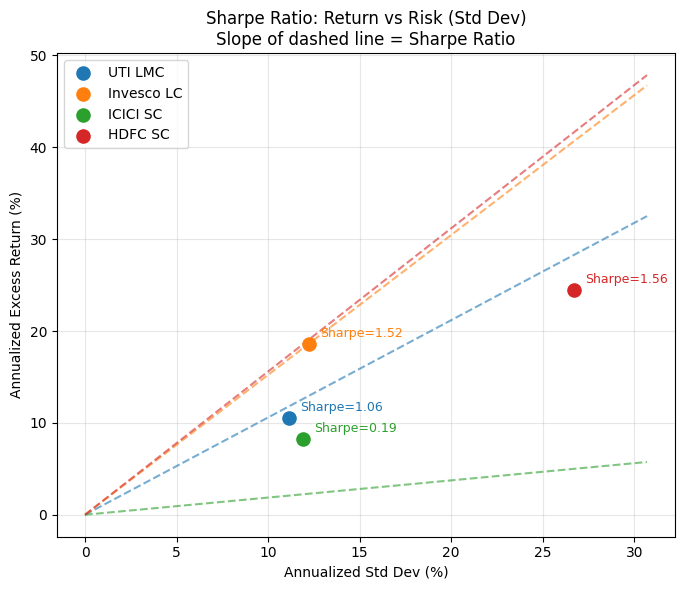
\includegraphics[width=0.7\linewidth]{sharpe.png}
    % \caption{Caption}
    % \label{fig:placeholder}
\end{figure}
    
\end{frame}

\begin{frame}{Treynor's Ratio Comparison}
\centering
\begin{figure}
    \centering
    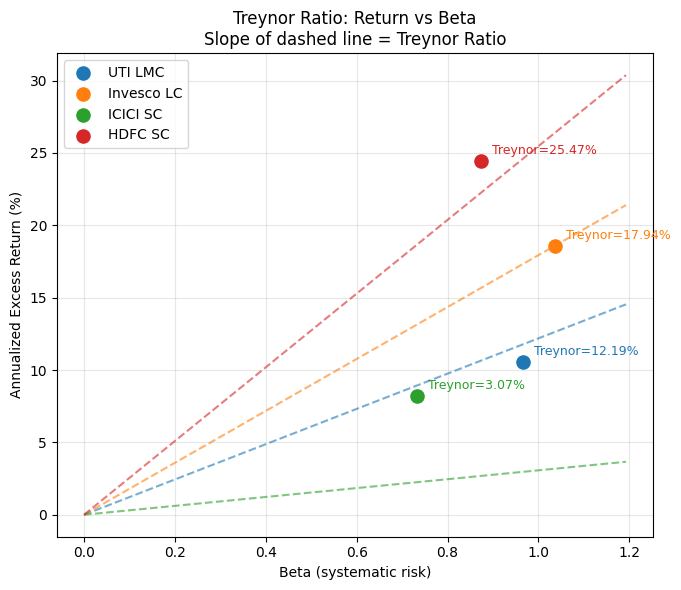
\includegraphics[width=0.7\linewidth]{treynor.png}
    % \caption{Caption}
    % \label{fig:placeholder}
\end{figure}
    
\end{frame}


\begin{frame}{Consolidated Factor Exposures (Carhart)}
\centering
\small
\begin{tabular}{l r r r r}
\toprule
\textbf{Factor} & \textbf{UTI LMC} & \textbf{Invesco LC} & \textbf{ICICI SC} & \textbf{HDFC SC} \\
\midrule
$\beta$ (Market) & \textcolor{posgreen}{0.9877} & \textcolor{posgreen}{1.0085 } & \textcolor{posgreen}{0.738} & \textcolor{posgreen}{0.81301} \\
$\delta$ (SMB) & $-$0.0000 & $-$0.0968 & 0.338 &  \textcolor{posgreen}{0.26391} \\
$\lambda$ (HML) & \textcolor{posgreen}{$-$0.0031} & 0.0684 &  \textcolor{posgreen}{$-$3.812} & 0.15294 \\
$\rho$ (MOM) & $-$0.0011 &  \textcolor{posgreen}{0.2807} & 0.224 & 0.03707 \\
$\alpha$ & $-$0.0001 & $-$0.0000 & \textcolor{posgreen}{1.521} &  \textcolor{posgreen}{0.001551} \\
$R^2$ & 0.9451 & 0.9288 & 0.9402 & 0.97123 \\
\bottomrule
\end{tabular}

\vspace{0.8em}
% \footnotesize
% \textit{ICICI source slides report factor coefficients and $R^2$ only; intercept, std.\ errors, and t-stats are not reported. HDFC figures are from the supplied July 2026 four-factor regression. Invesco content is unchanged.}
\end{frame}


% %% ===================================================================
% \section{Conclusion}
% %% ===================================================================

\begin{frame}{}
    \centering
    \vspace{2em}
    {\Huge Thank You}

    \vspace{1.5em}
    {\large Questions?}

    \vspace{2em}
    {\small Neeraja, Lokesh, Ajith, \& Balaji}
\end{frame}


\end{document}